\section{Iteración 2}

Una vez que ya tenemos conocimiento extraido de las entrevistas hay que plasmarlo.
Para ello se obtendrán reglas mediante las cuales podamos tomar una decisión, es decir,
crearemos un arbol de decicisión el cúal sea capaz de llevarnos a una táctica.

Para ello crearemos reglas simples, mediante las cuales con una serie de entradas,
obtendremos una salida. Esta salida puede tener diversas formas. Puede ser una decisión final
o la decisión de un camino intermedio para discernir si elegir una vía u otra.
Estas reglas deberán ser supervisadas por el experto, ya que estas simularan su decisión.

La creación de estas reglas llevarán a un prototipo de sistema experto, el cual será
la primera versión que podrá ser probada en un entorno local para ver si su uso aumenta
el porcentaje de victorias, además del número de tocados dados y a su vez, disminuir el
número de tocados recibidos.

Para ello se empezará con la creación de reglas básicas, como las de la primera entrevista. Esto
nos dará un arbol de decisión que podrá ser ampiable en todo momento.

El primer paso para crear dicho arbol será tener claro cual es el proceso en la toma de decisión.
Para ello se ha creado el diagrama, el cúal ha sido corroborado por el experto. Dicho diagrama
se puede observar en la figura 5.4.

\begin{figure}[htb]
  \centering
    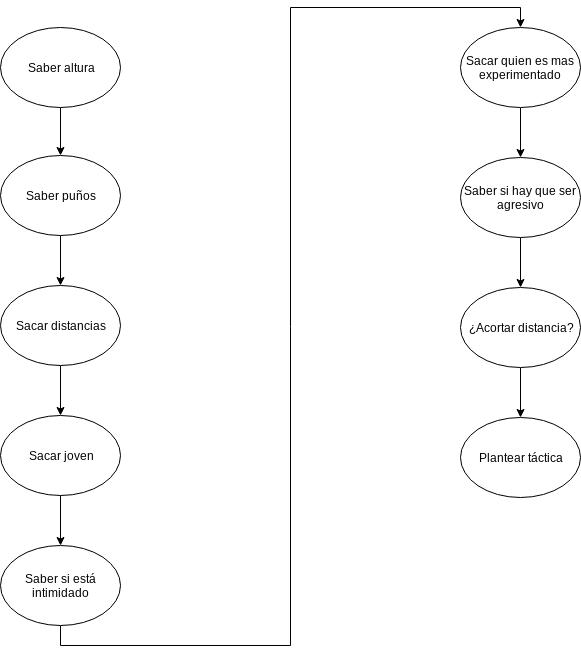
\includegraphics[width=0.8\linewidth]{mapaConocimiento1}
  \caption[Esquema toma decisión]{Esquema toma decisión}
  \label{fig:Esquema toma decisión}
\end{figure}


Con el arbol de decisiones resumido, se elaboraron los sub-arboles para cada uno de los casos.
Estos árboles han sido implantados como diagramas, los cuales se pueden ver en las figuras
5.5 (experiencia), 5.6 (distancia), 5.7 (agresividad), 5.8 (acortar distancia) y
5.9 (hierro y segunda intención).


\begin{figure}[htb]
  \centering
    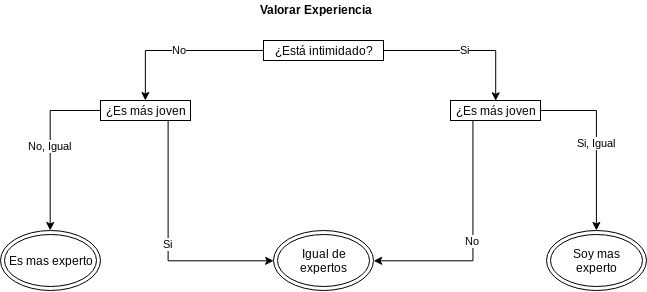
\includegraphics[width=0.8\linewidth]{MapaConocimientoExperiencia}
  \caption[Arbol decisión experiencia]{Arbol decisión experiencia}
  \label{fig:Arbol decisión experiencia}
\end{figure}

\begin{figure}[htb]
  \centering
    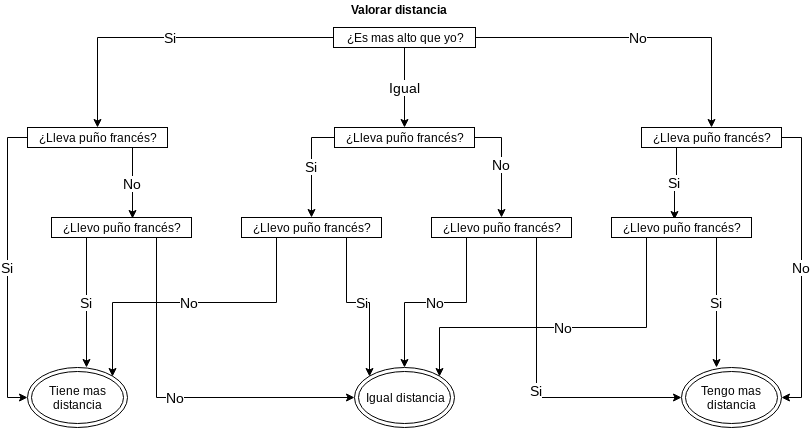
\includegraphics[width=0.8\linewidth]{MapaConocimientoDistancia}
  \caption[Arbol decisión distancia]{Arbol decisión distancia}
  \label{fig:Arbol decisión distancia}
\end{figure}


\begin{figure}[htb]
  \centering
    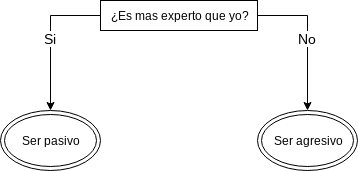
\includegraphics[width=0.8\linewidth]{MapaConocimientoAgresividad}
  \caption[Arbol decisión agresividad]{Arbol decisión agresividad}
  \label{fig:Arbol decisión agresividad}
\end{figure}


\begin{figure}[htb]
  \centering
    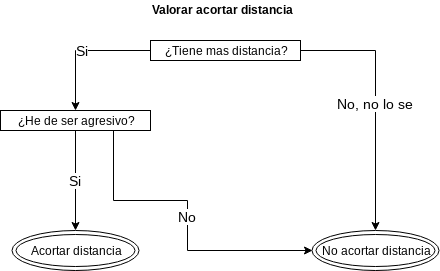
\includegraphics[width=0.8\linewidth]{MapaConocimientoAcortarDistancia}
  \caption[Arbol decisión acortar distancia]{Arbol decisión acortar distancia}
  \label{fig:Arbol decisión acortar distancia}
\end{figure}


\begin{figure}[htb]
  \centering
    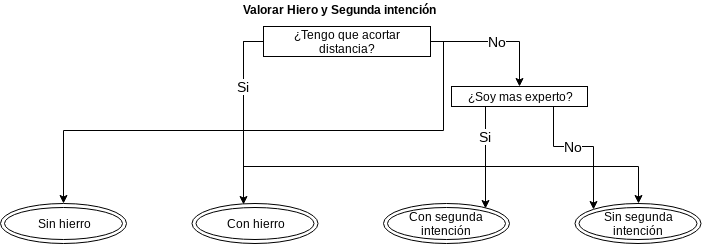
\includegraphics[width=0.8\linewidth]{MapaConocimientoHierroSIntencion}
  \caption[Arbol decisión hierro y segunda intención]{Arbol decisión hierro y segunda intención}
  \label{fig:Arbol decisión hierro y segunda intención}
\end{figure}



